%%%%\documentclass[10pt,a4paper]{article}
%%\documentclass[10pt,a4paper]{scrreprt}
%%\usepackage[utf8]{inputenc}
%%\usepackage{amsmath}
%%\usepackage{amsfonts}
%%\usepackage{amssymb}
%%\usepackage{graphicx}
%%\usepackage[left=2cm,right=2cm,top=2cm,bottom=2cm]{geometry}
%%\usepackage{natbib}
%%
%%\usepackage{bm}
%%
%%\usepackage{pythonhighlight}
%%
%%% integral d
%%\newcommand{\myd}{\;\mathrm{d}}
%%% overbar
%%\newcommand{\overbar}[1]{\mkern 1.5mu\overline{\mkern-1.5mu#1\mkern-1.5mu}\mkern 1.5mu}
%%
%%\author{Yi Hu}
%%\title{Homogenization for Multi Field Modelling}
%%\subtitle{Part I: Theories and FEniCS}
%%\begin{document}
%
%\maketitle
%\tableofcontents
%
%%%\documentclass[10pt,a4paper]{article}
%\documentclass[10pt,a4paper]{scrartcl}
%%\documentclass[10pt,a4paper]{scrreprt}
%\usepackage[utf8]{inputenc}
%\usepackage{amsmath}
%\usepackage{amsfonts}
%\usepackage{amssymb}
%\usepackage{graphicx}
%\usepackage[left=2cm,right=2cm,top=2cm,bottom=2cm]{geometry}
%\author{Yi Hu}
%\title{Homogenization for Multi Field Modelling}
%\subtitle{Part I: Theories and FEniCS}
%
%\begin{document}

\begin{abstract}
In this student project, Homogenization Method is utilized to investigate behaviour of composites under multiple fields. Many applications can be found in the field of Material Modelling, specifically for coupled problems of composites, e.g. Elastroactive Polymers. As for implementation, a novel Finite Element framework, FEniCS, is investigated. FEniCS is a collection of libraries and modules, which uses Python (or C++) as its interface language. The most important feature about FEniCS is its specialization in code generation with respect to bilinear forms, linear forms and function spaces in the formulation of computational problems, which can translate the mathematical language directly into codes and accelerates the trial process of new models and new computation methods. Moreover, Python make the implementation of a problem even faster, as it is a dynamical language for prototyping. In the framework of FEniCS a Unit Cell module is realized, where the calculation (include homogenized properties) of composites in micro scale under multiple fields could be performed.

\end{abstract}


%\end{document}
%

%
%%%\documentclass[10pt,a4paper]{article}
%\documentclass[10pt,a4paper]{scrreprt}
%\usepackage[utf8]{inputenc}
%\usepackage{amsmath}
%\usepackage{amsfonts}
%\usepackage{amssymb}
%\usepackage{graphicx}
%\usepackage[left=2cm,right=2cm,top=2cm,bottom=2cm]{geometry}
%\author{Yi Hu}
%\title{Homogenization for Multi Field Modelling}
%\subtitle{Part I: Theories and FEniCS}
%
%\begin{document}

\chapter{Introduction}

Composites play an important role in engineering, as they combine the advantages of each components in materials. They finds many applications in the field of Civil Engineering, Aerospace Engineering, etc. In order to understand composites thoroughly, experiments and simulations are accomplished. The current work specialized in the simulation of composites.

A multi scale model is conducive in modelling, where the deformation in small scale will be reflected in the corresponding macro scale. Micro structures in composites are essential for their properties. Material behaviours are determined by these micro structures. If an energy function is used to describe the composites, material components and geometry configuration in micro scale governs the material energy function. Under this condition, an appropriate energy function is sought after. However, the exact expression for composites under different loading and with various inclusion geometry is hard to obtain. Hence the consideration shift to acquire this description on the fly, i.e. to embed the result of micro scale simulation into macro scale simulation. From a practical perspective, models in multiple scales would lead to full understanding of composite, which will in return be beneficial for material design. Moreover, in computing scale separation would benefit from various computing techniques such as parrellelization and model reduction. These techniques would possibly boost the efficiency of computation. 

Intuitively a full simulation can be realized, where micro structures and different materials would be represented explicitly in the simulated object. This results in a tremendous many degrees of freedom consuming large amount of computation resources. Hence a full simulation accounting for all the micro structures and inclusions is not an efficient way.

In this work Homogenization Method is used to achieve multi scale modelling. The key task of homogenization is to calculate homogenized parameters for macro scale model, which is mainly based on the micro scale result. The formulation of homogenized parameters is carried out through material energy. Using material energy in the formulation is of great importance, as it simplifies the derivation of equilibrium and unifies the calculation of homogenized parameters. In the case of composites in multiple fields, energy formulation will result in relative simple formulation in the homogenized context. 

To avoid the lengthy derivation of equations for coupled fields, calculation under FEniCS framework is realized. Its strength lies in the field of coupled problem, which will be seen in the later chapter. 

The whole report will fall into two parts. The first part concentrates on the theory basics of simulation, while the second part focus more on the derivation and implementation for the composite simulation under multiple fields. Numerical examples and summary are given in the end of this report.

%\end{document}

%
%%%\documentclass[10pt,a4paper]{article}
%\documentclass[10pt,a4paper]{scrreprt}
%\usepackage[utf8]{inputenc}
%\usepackage{amsmath}
%\usepackage{amsfonts}
%\usepackage{amssymb}
%\usepackage{graphicx}
%\usepackage[left=2cm,right=2cm,top=2cm,bottom=2cm]{geometry}
%
%\usepackage{bm}
%
%% integral d
%\newcommand{\myd}{\;\mathrm{d}}
%% overbar
%\newcommand{\overbar}[1]{\mkern 1.5mu\overline{\mkern-1.5mu#1\mkern-1.5mu}\mkern 1.5mu}
%
%\author{Yi Hu}
%\title{Homogenization for Multi Field Modelling}
%\subtitle{Part I: Theories and FEniCS}
%
%
%\begin{document}

\chapter{Homogenization Method}
The method used in the current work is Homogenization Method. It was proposed in 1970s by Babuska and collaborators, [ref: abdulle]. The main purpose of this method is to make use of the scale separation, in order to obtain a reduced PDE for the macroscopic problem. The macroscopic problem always contains the information from the according micro scale, and it is often represented as ``effective parameters''. These effective parameters are often calculated in the sense of ``averaging procedure'' or ``homogenization''. As for the micro scale problem, various types of problem arise. They could be solved with either finite difference or finite element method, other kinds of numerical methods could also be employed. An extensive review is from the book [ref: multiscale thomas y hou]. A more general framework, the Heterogeneous Multiscale Method (HMM), was proposed by Bjorn Engquist. This method extend the idea of homogenization and introduce generic methodology between macro scale and micro scale. An introductory review could be found in [ref: weinan e].

In this part the basic idea of Homogenization Method is presented with a one dimensional example. Then the application to the 3d elliptic PDE is briefly discussed. Hill Mandel requirements should be fulfilled in the energy conserving problem. Hence they are stated in the end of this part. We confine our discussion here mainly on the material possessing periodic structures. 

\section{Periodic Structures}
Periodicity appears frequently in composites, for instance material with fiber or particle reinforcement. The periodicity in these materials takes the form of periodic geometry and periodic materials. Concerning about material parameters they could be expressed with periodic functions of coordinates. For example, Young's Modulus can be written in the following form,
%
\begin{equation}
\label{eq:periodic 1}
\mathbb{C}(\mathbf{x}+\mathbf{Y}) = \mathbb{C}(\mathbf{x}).
\end{equation}
%

\section{Scale Separation}
When two scale problem is addressed, field variable could be expanded as follows, 
%
\begin{equation}
\label{eq:field epsi}
\mathbf{\Phi}^{\epsilon}(\mathbf{x}) = \mathbf{\Phi}^{0}(\mathbf{x},\mathbf{y}) + \epsilon\mathbf{\Phi}^{1}(\mathbf{x},\mathbf{y}) + \epsilon\mathbf{\Phi}^{2}(\mathbf{x},\mathbf{y}) + \cdots,
\end{equation}
%
In the above formula, $\mathbf{x}$ is the position vector of a point, which is deemed as the \textit{macroscopic} coordinate. $\mathbf{y}=\mathbf{x}/\epsilon$ is a \textit{microscopic} coordinate, which stands for \textit{rapid} oscillation. The physical nature of the right hand side is the decomposition of macro scale dependency and micro scale dependency with respect to reference cell. The purpose of setting $\mathbf{y}=\mathbf{x}/\epsilon$ is achieving a closed form expressed with the original coordinates. The ratio $\epsilon$ means that the quantity will vary $1/\epsilon$ faster in microscopic level. When $\epsilon$ goes to $0$, functions $\mathbf{\Phi}^{0}(\mathbf{x}, \mathbf{y}), \mathbf{\Phi}^{1}(\mathbf{x}, \mathbf{y}), \cdots$ are smooth in $\mathbf{x}$ and $\mathbf{Y}$-periodic in $\mathbf{y}$.

The characteristic of field variable can be viewed in the diagram [figure: scale decomposition]

\section{One Dimensional Problem}
Many books and review papers list one dimensional problem, such as [ref: ciorsanescu]. Here we briefly go through one dimensional elasticity problem. More detailed derivation could be referred to [ref: B.hassani].

The governing equations such as the equilibrium and Hooke's law are,
\begin{equation}
\left\{
\begin{array}{l}
\dfrac{\partial \sigma^{\epsilon}}{\partial x} + \gamma^{\epsilon} = 0 \\
\sigma^{\epsilon} = E^{\epsilon} \dfrac{\partial u^{\epsilon}}{\partial x},
\end{array}
\right.
\end{equation}

Noting that $\epsilon$ in superscript represents its periodic property. $\gamma^{\epsilon}$ is the body weight of material. If $E^{\epsilon}$ and $\gamma^{\epsilon}$ are uniform in macro coordinate and only differ inside each cell, then the following relation holds,
\begin{equation}
E^{\epsilon}(x,x/\epsilon)=E^{\epsilon}(x/\epsilon)=E(y),
\end{equation}
The relation with respect to body weight is likewise. Utilizing the double scale expansion referring to (\ref{eq:field epsi}) it follows that,
\begin{equation}
\left\{
\begin{array}{l}
u^{\epsilon}(x) = u^{0}(x,y) + \epsilon u^{1}(x,y) + \epsilon^{2} u^{2}(x,y) + \cdots \\
\sigma^{\epsilon}(x) = \sigma^{0}(x,y) + \epsilon \sigma^{1}(x,y) + \epsilon^{2} \sigma^{2}(x,y) + \cdots,
\end{array}
\right.
\end{equation}

After substitution and equating the according terms, we have
\begin{equation}
\label{eq: to simp 1}
\left\{
\begin{array}{l}
0 = E(y)\left( \dfrac{\partial u^{0}}{\partial y} \right) \\
\sigma^{0} = E(y) \left( \dfrac{\partial u^{0}}{\partial x} + \dfrac{\partial u^{1}}{\partial y} \right) \\
\sigma^{1} = E(y) \left( \dfrac{\partial u^{1}}{\partial x} + \dfrac{\partial u^{2}}{\partial y} \right),
\end{array}
\right.
\end{equation}
and
\begin{equation}
\label{eq: to simp 2}
\left\{
\begin{array}{l}
\dfrac{\partial \sigma^{0}}{\partial y}=0 \\
\dfrac{\partial \sigma^{0}}{\partial x} + \dfrac{\partial \sigma^{1}}{\partial y} + \gamma(y) = 0, 
\end{array}
\right.
\end{equation}
Simplification of (\ref{eq: to simp 1}) and (\ref{eq: to simp 2}) yields
\begin{equation}
\label{eq: sigma 0}
\sigma^{0}(x) = \left(Y/\int_{Y} \dfrac{\myd{y}}{E(y)} \right) \dfrac{\myd{u^{0}(x)}}{\myd{x}}.
\end{equation}
Define the \textit{homogenized modulus of elasticity} as follows,
\begin{equation}
E^{H} = 1/ \left( \dfrac{1}{Y} \int_{0}^{Y} \dfrac{\myd{\eta}}{E(\eta)}\right) .
\end{equation}
Then the original problem is transformed to
\begin{equation}
\label{eq: homo 1d}
\left\{
\begin{array}{l}
\sigma^{0}(x) = E^{H} \dfrac{\myd{u^{0}(x)}}{\myd{x}} \\
\dfrac{\myd{\sigma^{0}}}{\myd{x}} + \bar{\gamma} = 0,
\end{array}
\right.
\end{equation}
where $\bar{\gamma}=1/Y \int_{Y} \gamma(y)$ is the average of $\gamma$ inside the cell. From (\ref{eq: homo 1d}) the differential equation for displacement holds as
\begin{equation}
\dfrac{\myd^2 u^{0}(x)}{\myd{x^{2}}} = -\dfrac{\bar{\gamma}}{E^{H}}
\end{equation}
Regarding the boundary conditions on both ends deliver the result
\[u(x) = -\dfrac{\bar{\gamma}}{E^{H}} \dfrac{x^{2}}{2} + \dfrac{\bar{\gamma}}{E^{H}} Lx \]

\section{General Elliptical PDE}
If a general PDE for three dimensional problem is taken into account, it would be more intricate, as the solution is often sought in the sense of weak form. In this circumstance a homogenized weak form is considered instead of the homogenized differential operator. Then the limit of homogenized weak form should converge to the weak form without homogenization, which is called \textit{G-convergence}, [ref: a comparison, u michi]. As for the case of elasticity tensor in the sense of differential operator G-convergence is the following,
\begin{equation}
\label{eq: G conv}
\lim_{\epsilon \to 0} \dfrac{\partial}{\partial x_{i}} \left[ C^{\epsilon}_{ijkl} \dfrac{\partial u^{\epsilon}_{k}}{\partial x_{l}} \right] \rightarrow \dfrac{\partial}{\partial x_{i}} \left[ \bar{C}_{ijkl} \dfrac{\partial u_{k}}{\partial x_{l}} \right]
\end{equation}
A quick overview of the general problem is given in the review [ref: hassani]. Several key points of the general problem are listed here. With the notation of general elliptical operator using 
\begin{equation}
\mathcal{A}^{\epsilon} = \dfrac{\partial}{\partial x_{i}} \left( a_{ij}(\mathbf{y}) \dfrac{\partial}{\partial x_{j}} \right).
\end{equation}
general problem could then be described as,
\begin{equation}
\left\{
\begin{array}{ll}
\mathcal{A}^{\epsilon} \mathbf{u^{\epsilon}}= \mathbf{f} & \text{in} \ \Omega \\
\mathbf{u}^{\epsilon} = \mathbf{0} & \text{on} \ \partial \Omega
\end{array}
\right.
\end{equation}
Employing the double scale expansion for both the field variable $\mathbf{u}^{\epsilon}$ and the differential operator $\mathcal{A}^{\epsilon}$, namely (notice that chain rule is applied when differentiating)
\begin{equation}
\left\{
\begin{array}{l}
\mathbf{u}^{\epsilon}(\mathbf{x}) = \mathbf{u}^{0}(\mathbf{x},\mathbf{y}) + \epsilon \mathbf{u}^{1}(\mathbf{x},\mathbf{y}) + \epsilon^{2} \mathbf{u}^{2}(\mathbf{x},\mathbf{y}) + \cdots \\
\mathcal{A}^{\epsilon} = \dfrac{1}{\epsilon^{2}} \mathcal{A}^{1} + \dfrac{1}{\epsilon} \mathcal{A}^{2} + \mathcal{A}^{3}
\end{array}
\right.
\end{equation}
Here $\mathcal{A}^{1}, \mathcal{A}^{2}, \mathcal{A}^{3}$ is defined as follows
\[
\mathcal{A}^{1} = \dfrac{\partial}{\partial y_{i}} \left( a_{ij}(\mathbf{y}) \dfrac{\partial}{\partial y_{j}} \right); \
\mathcal{A}^{2} = \dfrac{\partial}{\partial y_{i}} \left( a_{ij}(\mathbf{y}) \dfrac{\partial}{\partial x_{j}} \right) + \dfrac{\partial}{\partial y_{i}} \left( a_{ij}(\mathbf{y}) \dfrac{\partial}{\partial x_{j}} \right); \
\mathcal{A}^{3} = \dfrac{\partial}{\partial x_{i}} \left( a_{ij}(\mathbf{y}) \dfrac{\partial}{\partial x_{j}} \right).
\]
Substitution with the above differential operators and comparing with the according terms it follows
\begin{equation}
\label{eq: eq group}
\left\{
\begin{array}{l}
\mathcal{A}^{1} \mathbf{u}^{0} = \mathbf{0} \\
\mathcal{A}^{1} \mathbf{u}^{1} + \mathcal{A}^{2} \mathbf{u}^{0} = \mathbf{0} \\
\mathcal{A}^{1} \mathbf{u}^{2} + \mathcal{A}^{2} \mathbf{u}^{1} + \mathcal{A}^{3} \mathbf{u}^{0} = \mathbf{f}.
\end{array}
\right.
\end{equation}
Referring [ref: cioranescu] it is known that if a $\mathbf{Y}$-periodic function $u$ has a unique solution in terms of $\mathcal{A}^{1}$ operator, i.e. 
\begin{equation}
\mathcal{A}^{1} \mathbf{u} = \mathbf{F} \quad \text{in the reference cell}.
\end{equation}
Then the right hand side of the above equation, $\mathbf{F}$ should satisfy 
\begin{equation}
\overbar{\mathbf{F}} = \dfrac{1}{|Y|}\int_{Y} \mathbf{F} \myd{\mathbf{y}} = \mathbf{0}.
\end{equation}
Applying this proposition to (\ref{eq: eq group}) several times the field variable could be expressed with the following form,
\begin{equation}
\mathbf{u}^{1}(\mathbf{x}, \mathbf{y}) = \chi^{i}(\mathbf{y}) \dfrac{\partial \mathbf{u}(\mathbf{x})}{\partial x_{j}} + \mathbf{\xi} (\mathbf{x})
\end{equation}
Function $\chi^{i}(\mathbf{y})$ is local solution of the problem, which has $\mathbf{Y}$-periodic property. The local problem is
\begin{equation}
\mathcal{A}^{1} \mathbf{\chi}^{j}(\mathbf{y}) = \dfrac{\partial a_{ij}(\mathbf{y})}{\partial y_{i}} \quad \text{in the reference cell}.
\end{equation}
Hence the macro scale problem (homogenized problem) can be written as
\begin{equation}
\mathcal{A}^{H} \mathbf{u} = \mathbf{f},
\end{equation}
with
\begin{equation}
\mathcal{A}^{H} = a^{H}_{ij} \dfrac{\partial^{2}}{\partial x_{i} \partial x_{j}}.
\end{equation}
%
And the effective coefficients are related with the solution of micro scale problem,
\begin{equation}
a^{H}_{ij} = \dfrac{1}{|Y|} \int_{Y} \left( a_{ij}(\mathbf{y}) + a_{ik}(\mathbf{y}) \dfrac{\partial \chi^{j}}{\partial y_{k}} \right) \myd{\mathbf{y}}
\end{equation}

%--------------------------------
\section{Hill-Mandel Condition}
After introducing the general mathematical concepts about homogenization methods, we move to its application in material modelling. In this case a Representative Volume Element (RVE) is always investigated. Homogenization of the coefficients is then obtained through calculation on RVE. As RVE represents a material in the micro scale, the behaviour of RVE should resemble the material in this scale. Therefore the model for micro scale should be able to capture such features, for instance the continuum mechanical equilibrium of composites in the micro scale. Besides the boundary condition of micro scale model should also be compatible with macro scale. The Hill-Mandel condition needs to be fulfilled [ref: r.hill 1952 from gluege]

The Hill-Mandel condition states that the total stress power on the micro scale should be equal to the stress power at relevant point on the macro scale. For small strain, the following equation holds,

\begin{equation}
\left< \bm{\sigma} \cdot \dot{\bm{\varepsilon}} \right> = \left< \bm{\sigma} \right> \cdot \left< \dot{\bm{\varepsilon}} \right>,
\end{equation}
where $\left< \cdot \right>$ means averaging of the considered variable.

%\end{document}
%
%
%
%
%
%
%
%
%
%
%
%
%
%
%
%
%
%
%

%
%%%\documentclass[10pt,a4paper]{article}
%\documentclass[10pt,a4paper]{scrreprt}
%\usepackage[utf8]{inputenc}
%\usepackage{amsmath}
%\usepackage{amsfonts}
%\usepackage{amssymb}
%\usepackage{graphicx}
%\usepackage[left=2cm,right=2cm,top=2cm,bottom=2cm]{geometry}
%\usepackage{natbib}
%\usepackage{bm}
%
%\usepackage{pythonhighlight}
%
%% integral d
%\newcommand{\myd}{\;\mathrm{d}}
%% overbar
%\newcommand{\overbar}[1]{\mkern 1.5mu\overline{\mkern-1.5mu#1\mkern-1.5mu}\mkern 1.5mu}
%
%\author{Yi Hu}
%\title{Homogenization for Multi Field Modelling}
%\subtitle{Part I: Theories and FEniCS}
%
%\begin{document}

\chapter{Finite Element Framework FEniCS}

FEniCS project was started at University of Chicago and Charmers University of Technology in 2003. The name ``FEniCS" consists ``FE", ``Finite Element" and ``CS", ``Computational Software". ``ni" makes the name sound like ``phenix". It is a collection of packages that make the best of each package to realize Computational Mathematical and Modelling. The main interface language of FEniCS is Python, which is a fast language for prototyping, while the most of codes and libraries are implemented in C++, whose efficiency in computing stands out. Various linear algebra backends and parallelization allow FEniCS boost in speed. As for modelling, UFL (Unified Form Language) and FFC (FEniCS Form Compiler) allow the direct translation of mathematical formulation such as linear form and bilinear form into symbolic codes. It can be regarded as the language of modelling, which simplifies the modelling process to a large extent \citep{kirby2006compiler}.

This part concentrates on the introduction of FEniCS. Firstly the work flow and components of FEniCS will be presented. Then the most simple example is given in order to clarify its efficiency in modelling. At last some key features of FEniCS is listed and discussed, which provides the flexibility in simulations.

%--------------------------------
\section{The Structure of FEniCS}
The work flow of FEniCS can be described with the following diagram. It is seen that the whole process is decomposed into three major parts. Each part represents one or several functionalities. For form compiler UFL language is involved. With the help of form compiler (FFC), C++ code of the whole model is obtained. Till this point the mathematical derivation, which is the weak form of a PDE in most cases, is converted into pure symbolic efficient C++ codes. The interface between symbolic codes and numerical codes is called UFC (Unified Form-assembly Code). It works as a fixed interface that achieve efficient assembling of finite elements \citep{wells2012automated}.

\begin{figure}[h]
\center
\label{fig: fenics blocks}
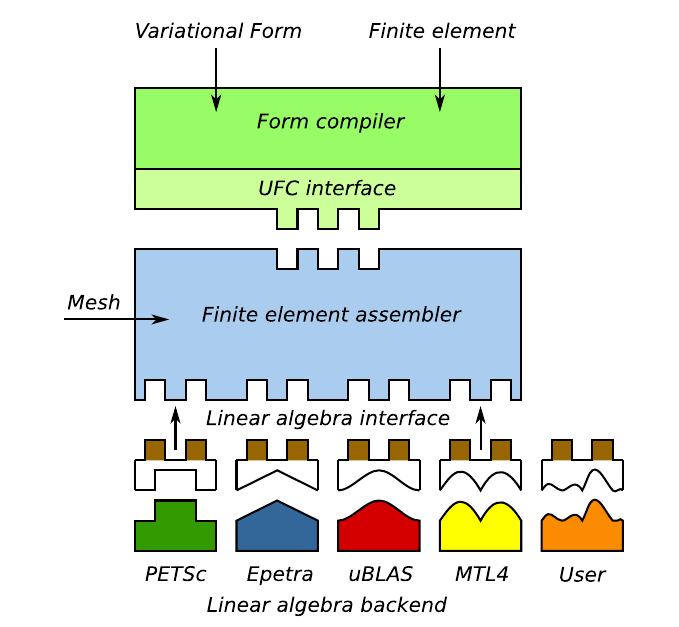
\includegraphics[width=0.6\linewidth]{../pics/fenics_building_blocks.png}
\caption{Building Blocks of FEniCS \citep{wells2012automated}}
\end{figure} 

Numerical algorithms enter after the UFC interface. The main package that carries the numerical algorithm is DOLFIN. DOLFIN's task is to wrap functionalities of each components and their interactions. The user interface of DOLFIN is Python, where object oriented programming can be followed in a easy fashion.  

Other building blocks such as mshr for geometrical modelling and mesh generation, and FIAT (FInite element Automatic Tabulator) for automatic finite element generation for arbitrary orders. Linear algebra backends work as add-ons for FEniCS, which provides the possibility of extension. The visualization package in use is VTK, a substitute of the old one, Viper. The output files could be in various formats. Therefore software like ParaView could apply in terms of visualization. The full structure of FEniCS can be viewed in the following diagram.

\begin{figure}[h]
\center
\label{fig: fenics map}
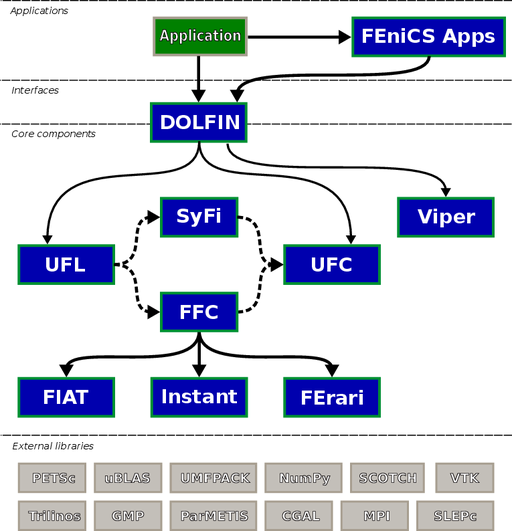
\includegraphics[width=0.5\linewidth]{../pics/fenics_map.png}
\caption{Components of FEniCS \citep{wells2012automated}}
\end{figure} 

%--------------------------------
\section{Simple Poisson Problem}
An implementation of simple Poisson problem is presented in the official tutorial of FEniCS. This example is reproduced here to give a quick overview of the usage and convince its simplicity in modelling \citep{wells2012automated}.

\begin{python}
from dolfin import *

# Create mesh and define function space
mesh = UnitSquareMesh(6, 4)
V = FunctionSpace(mesh, 'Lagrange', 1)

# Define boundary conditions
# Value function for boundary condition x[0]->x, x[1]->y
u0 = Expression('1 + x[0]*x[0] + 2*x[1]*x[1]')
# Mark boundary
def u0_boundary(x, on_boundary):
    return on_boundary
# Add Dirichlet boundary condition
bc = DirichletBC(V, u0, u0_boundary)

# Define variational problem
u = TrialFunction(V)
v = TestFunction(V)
f = Constant(-6.0)
# Bilinear Form
a = inner(nabla_grad(u), nabla_grad(v))*dx
# Linear Form
L = f*v*dx

# Compute solution
u = Function(V)
solve(a == L, u, bc)

# Plot solution
plot(u, interactive = True)

# Dump solution to file in VTK format
file = File('poisson.pvd')
file << u
\end{python}

As can be immediately seen in the code, the encapsulation of almost every functionality is well preserved in FEniCS. Moreover, the name of functions and classes are in good consistent with the mathematical language. The modelling always begins with defining its geometry and function space. This setting is similar with solving a PDE in weak form, where its domain and function spaces are usually given in condition. Geometry and mesh can also be imported using external files. Various formats are supported, such as \texttt{.msh} generated by \texttt{gmsh}. One thing to notice is that element type is defined when defining function space. As shown in the example \texttt{'Lagrange’}. The order of element is simply 1.

It follows with defining the boundary conditions such as Dirichlet boundary conditions. An \texttt{Expression} is a class holding the codes of creating a mathematical function in the domain. It is extensible with C++. Here we use it to define the boundary values. As for imposing this boundary condition, one need to mark the boundary first. Marking other boundary entities such as points, lines, and facets is the same with the provided code structure. \texttt{on\_boundary} is only a predefined marker that will return \texttt{True} when on the boundary.

The mathematical model of this problem is 
\begin{equation}
\label{eq: poisson}
\left\{
\begin{array}{ll}
-\Delta u(\mathbf{x})=0 & \text{in} \ \Omega \\
u(\mathbf{x})=u_{0} & \text{on} \ \partial \Omega .
\end{array}
\right.
\end{equation}
The according weak form can be written as
\begin{equation}
\label{eq: weak}
a(u,v) = L(v), \ \forall v \in \hat{V}
\end{equation}
with the bilinear form and linear form defined as
\[
a(u,v) = \int_{\Omega} \nabla{u} \cdot \nabla{v} \myd{\mathbf{x}}, \ L(v) = \int_{\Omega} fv \myd{\mathbf{x}}.
\]
The sought after function is $u$ in function space $V = \left\lbrace v \in H^{1}\left( \Omega \right) : v=u_{0} \  \text{on} \ \partial \Omega \right\rbrace$ and the according $\hat{V}$ is defined as $\hat{V} = \left\lbrace v \in H^{1}\left( \Omega \right) : v=0 \  \text{on} \ \partial \Omega \right\rbrace$. In the code the above mathematical model is conveniently expressed with \texttt{a\ =\ inner(nabla\_grad(u),\ nabla\_grad(v))*dx} and \texttt{L\ =\ f*v*dx}.

Next is the solving step, where one should redefine a new \texttt{Function} to hold the solution. Here overriding the above defined \texttt{u} is implemented. Post processing such as visualization of the result follows with \texttt{plot}. Output of the result is also standard with the listed commands.

The presentation of the simple Poisson problem serves as an introduction to the functionalities of FEniCS. To sum up, the implementation is in accordance with mathematical notation. Pre and post processing of the computation can be realized using handy functions supported by FEniCS. More useful features are discussed in the following section.

%--------------------------------
\section{Relevant Key Features}
When the problem becomes more complicated, there are more advanced and handy usage come into play. Here list only a few that appear in the material modelling and multi field problems.

First we explore the function space in FEniCS. There are several kinds of \texttt{FunctionSpace} in FEniCS. If a vector or tensor is used, \texttt{VectorFunctionSpace} or \texttt{TensorFunctionSpace} should be defined. More powerful usage is the \texttt{MixedFunctionSpace}, which receives a list of \texttt{FunctionSpace} and compose them together into a merged one. It is especially useful when multiple fields are accounted. When concerning about constructing function spaces, various function space families are available. Thanks to the general representation of function spaces arbitrary order of elements and a lot many types are possible. For very specific function space which requires periodicity \texttt{constrained\_type} keyword is set to be a periodic mapping. This mapping is derived from \texttt{SubDomain}. Much caution needs to be devoted into the definition of mapping, which can be observed in the corresponding code for material modelling.

\begin{python}
# Useful properties and variables for FunctionSpace definition
FS = FunctionSpace(mesh=some_mesh, family='Lagrange', degree=2, constrained_domain=some_defined_periodic_mapping)

# Vector and tensor function spaces
VFS = VectorFunctionSpace(mesh, 'Lagrange', 1)
TFS = TensorFunctionSpace(mesh, 'Hermite', 1)

# Merged function Space
MFS = MixedFunctionSpace([FS, VFS, TFS])
\end{python}

When it is concerned with multi field modelling, not only merged function but also split functions are required, since in the formulation different terms are calculated with different functions. A mixed function is generated with a \texttt{MixedFunctionSpace} and the corresponding component functions are obtained through \texttt{split} without losing dependency to the merged function. In the problem formulation it is often the case that inner product, outer product, derivative, and integral etc. are built. This is achieved easily with the help of UFL operators. Some of the operators such as \texttt{nabla\_grad()} and \texttt{inner()} are already mentioned above. One strength of FEniCS is that this formulation is not restricted in the vector and matrix, but applicable on tensors of higher order. The index notation representation is also valid in the formulation, namely \texttt{i,j,k,l}, obeying Einstein's summation convention. After the derivation a stiffness matrix is assembled with \texttt{assemble}. The usages are as follows.

\begin{python}
# Merged function space
MFS = MixedFunctionSpace([FS, VFS, TFS])

# Merged function and split functions
merged_f = Function(MFS)
(f, vf, tf) = split(merged_f)

# Integral
L = f*v*dx

# Derivative and its alternative
L_derivative = derivative(L, f, df)
L_diff = diff(L, f)

# Index notation
i, j, k, l = indices(4)
Energy = 0.5*F[i,j]*C_i_[i,j,k,l]*F[k,l]*dx

# Stiffness matrix, note that test function and trial function should be initiated first
f_test = TestFunction(FS)
f_trial = TrialFunction(FS)
a = f_test*C*t_trial*dx
K = assemble(a)
\end{python}

The last usage is particularly useful in composite modelling, i.e. defining different domains. The definition is also not complicated. Subdomains are defining through subclassing of \texttt{SubDomain}. Overriding its member method \texttt{inside()} gives the condition to distinguish whether it is in the corresponding subdomain or not. In integral the differentials are set accordingly to the subdomain.

\begin{python}
# Inclusion definition
class Inclusion(SubDomain):
    def inside(self, x, on_boundary):
        d = sqrt((x[0] - 0.5)**2 + (x[1] - 0.5)**2)
        return d<0.25 or near(d,0.25)

# Initiate an instance
circle = Inclusion()

# Set cell domains for integral
domains = CellFunction("size_t", mesh)
domains.set_all(0)
# Mark inclusion
circle.mark(domains,1)

# Integrate accordingly
dx = Measure('dx', domain=mesh, subdomain_data=domains)
Pi = psi_m*dx(0) + psi_i*dx(1)
\end{python}

%\end{document}

%
%%\documentclass[10pt,a4paper]{article}
%\usepackage[utf8]{inputenc}
%\usepackage{amsmath}
%\usepackage{amsfonts}
%\usepackage{amssymb}
%\usepackage{graphicx}
%\usepackage[left=2cm,right=2cm,top=2cm,bottom=2cm]{geometry}
%\usepackage{natbib}
%\author{Yi Hu}
%
%\begin{document}
\bibliographystyle{plain}
\bibliography{/home/yihu/studien_arbeit_fenics/report/part2/part2_ref.bib}
\nocite{*}
%\end{document}

%
%
%\end{document}